\documentclass[iop]{emulateapj}
%\documentclass[12pt,preprint]{aastex}
\bibliographystyle{apj}
\usepackage{graphicx}    % needed for including graphics e.g. EPS, PS
\usepackage{color}
%\usepackage{hyperref}
\newcommand{\Lsun}{L_{\odot}}
\newcommand{\Msun}{M_{\odot}}
\newcommand{\kms}{{\rm km} \, {\rm s}^{-1}}
\newcommand{\Mvir}{M_{\rm vir}}
\newcommand{\Rvir}{R_{\rm vir}}
\newcommand{\Mgas}{M_{\rm gas}}
\newcommand{\Mcold}{M_{\rm cold}}
\newcommand{\Mhot}{M_{\rm hot}}
\newcommand{\Mstar}{M_{\rm star}}
\newcommand{\Mgal}{M_{\rm gal}}
\newcommand{\NHI}{N_{\rm HI}}
\newcommand{\Msh}{M_{\rm sh}}
\newcommand{\CF}{f_{c}}
\newcommand{\CFR}{f_{c}(<\hspace{-0.7 ex}R)}
\newcommand{\MGII}{Mg$\,$II }

\newenvironment{inlinefigure}{
\def\@captype{figure}
\noindent\begin{minipage}{0.999\linewidth}\begin{center}}
{\end{center}\end{minipage}\smallskip}

\submitted{Draft 2015 Aug 31}

\begin{document}
%\title{REVEALING THE INVISIBLE. II. PLAYING TO LCOGT’S STRENGTHS: A PILOT HIGH-CADENCE MONITORING CAMPAIGN OF STRONG GRAVITATIONAL LENS HE0435}
%\title{A PILOT HIGH-CADENCE MONITORING CAMPAIGN OF STRONG GRAVITATIONAL LENS HE0435}
%\title{A Strong Gravitational Lens Time Delay with 15-Minute Precision}
\title{High-Precision Time Delays in Gravitational Lenses. II. A LCOGT Pilot on HE0435$-$1223}
\author{Leonidas A.\ Moustakas\altaffilmark{1}}
\author{Andrew Romero-Wolf\altaffilmark{1}}
\author{Curtis McCully\altaffilmark{2}}
\author{Todd Boroson\altaffilmark{2}}
\author{Aaron Bunch\altaffilmark{3}}
\author{Christopher Gonzalez\altaffilmark{4}}
\author{Francis-Yan Cyr-Racine\altaffilmark{1}}
\author{Charles Keeton\altaffilmark{5}}
\author{Frederic Courbin\altaffilmark{6}}

\altaffiltext{1}{JPL/Caltech, Pasadena, CA}
\altaffiltext{2}{LCOGT, Santa Barbara, CA}
\altaffiltext{3}{At Large}
\altaffiltext{4}{At Large}
\altaffiltext{5}{Rutgers University}
\altaffiltext{6}{EPFL}

\begin{abstract} 
  Accurate measurements of the delays in arrival time of photons
  between images in multiply-imaged time-varying sources such as
  strongly-lensed quasars opens new doors to astrophysical constraints
  on cosmological parameters, the structure of galaxies and their
  environments, and the nature of dark matter. The confidence level
  and accuracy of a time delay measurement in a given gravitational
  lens depends on a combination of photometric precision,
  observational cadence, and total campaign duration that matches the
  variability properties of the lensed quasar, and the value of the
  intrinsic time delay.  While time delays have been measured for
  nearly fifty image-pairs across nearly twenty lensed quasar systems,
  the absolute uncertainty to date is rarely better than $\sim1$\,day.
  To unlock the greatest potential of time delay probes, a greater
  than 100-fold improvement in precision is needed. We have completed
  a pilot ground-based campaign with the Las Cumbres Observatory
  Global Telescope network, monitoring the four-image lensed quasar
  HE\,$0435-1223$ with 420 contiguous five-minute observations. The
  integration time was selected to strike a balance between the
  photon-based signal to noise, the variations in the quasar light
  curve we aimed to be sensitive to, and the seeing quality.  We
  report on a systematic analysis of the observations, including
  optimized Bayesian-inference based point-spread-function photometry,
  the level of stability in the calibration and the sources of
  photometric and systematic uncertainties, and on the
  Bayesian-inference derived time delay analysis of the data. We find
  a firm photometric uncertainty floor of $\sim3-10$\%, a reasonable
  performance of the inference-based PSF fitting algorithm, and a
  {\bf XX}\% confidence level in a new measurement of the time delay
  between the leading and second images of the system (M1$-$M2) of
  $6.3\pm0.3$\,hours.  
\end{abstract}
\keywords{methods: statistical --- time --- gravitational lensing ---
  gravitational lens: HE0435$-$1223} 

% Kochanek+ 2006 give ΔtAC = −2.10+0.78 days = 
%  A time delay
%   measurement relies on the combination of photometric precision and
%   accuracy, cadence and campaign length of the photometric precision, including
%   controlling the systematic uncertaintWe report on a pilot
%   program Since the first 
% 
% makes possible measurements of Hubble's
%   constant as well as other cosmological parameters, as well as being
%   sensitive to the statistical contribution of substructures within
%   the lensing object.  time delay measurements made to date are from
%   ground-based monitoring observations, and generally We report on
% 
%  The thermal and interaction properties of the dark matter particle
%   encode information on astronomical structures.  Sub-galactic
%   structure within massive galaxies has the potential of being an
%   especially sensitive tracer, if a robust measurement can be made
%   down to sub-dwarf galaxies mass scales. Strong gravitational lenses
%   offer the opportunity to measure such structures at cosmologically
%   large distances, within lensing galaxies. Each lensing quantity that
%   connects to an observable in a gravitational lens, i.e. the
%   magnification, the spatial configuration, and the travel time for
%   light from a lensed source to the observer, has a specific (and
%   different) connection to the influence of substructure within the
%   galaxy or along the line of sight. The time-delays, the differences
%   in the arrival time for light between lensed images in such an
%   object, have great sensitivity to substructures. The substructure
%   perturbations affect images in different ways that allow them to be
%   related to substructure robustly, while the combination of all
%   supporting observations constrain the "macro" lens and environment
%   simultaneously, through state of art Inference-based lens modeling
%   that we have developed. The time delay precision necessary is a few
%   hours -- an order of magnitude better than what has been achieved
%   with ground based campaigns to date. We propose a pilot program,
%   uniquely possible with LCOGT, on two ideal gravitational lenses,
%   with coordinated complementary observations with ESO/VLT.  
% \\
% We measure the time delay between images M1 and M2 to be
% $6.3\pm0.25$\,hours.  

%%%%%%%%%%%%%%%%%%%%%%%%%%%%%%%%%%%%%%%%%%%%
\section{Introduction}

In strong gravitational lensing, light from a distant source is
focused into multiple images, with a geometry and detailed properties
that depend on the relative distances and line of sight alignment, the
distribution and structure of matter in and near the lensing object
and along the line of sight, and on the luminosity-fluctuations (if
any) of the lensed source. The excess arrival time of photons to an
observer is expressed as
\begin{equation}
\tau({\mathbf x}) = 
{{1+z_l}\over{c}}
{{D_lD_s}\over{D_{ls}}} 
\left[
{{1}\over{2}} |{\mathbf x} - {\mathbf u}|^2 - \phi({\mathbf x})
\right], \label{eq:arrivaltime}
\end{equation}
where light from the source at positions ${\mathbf u}$ is deflected by
the projected potential $\phi({\mathbf x})$ at image positions
${\mathbf u}$. The distances to the lens, to the source, and between
the lens and the source ($D_l$, $D_s$, and $D_{ls}$, respectively) are
angular-diameter distances, and $z_l$ is the redshift of the
lens. 

\begin{inlinefigure}
\begin{center}
  \resizebox{\textwidth}{!}{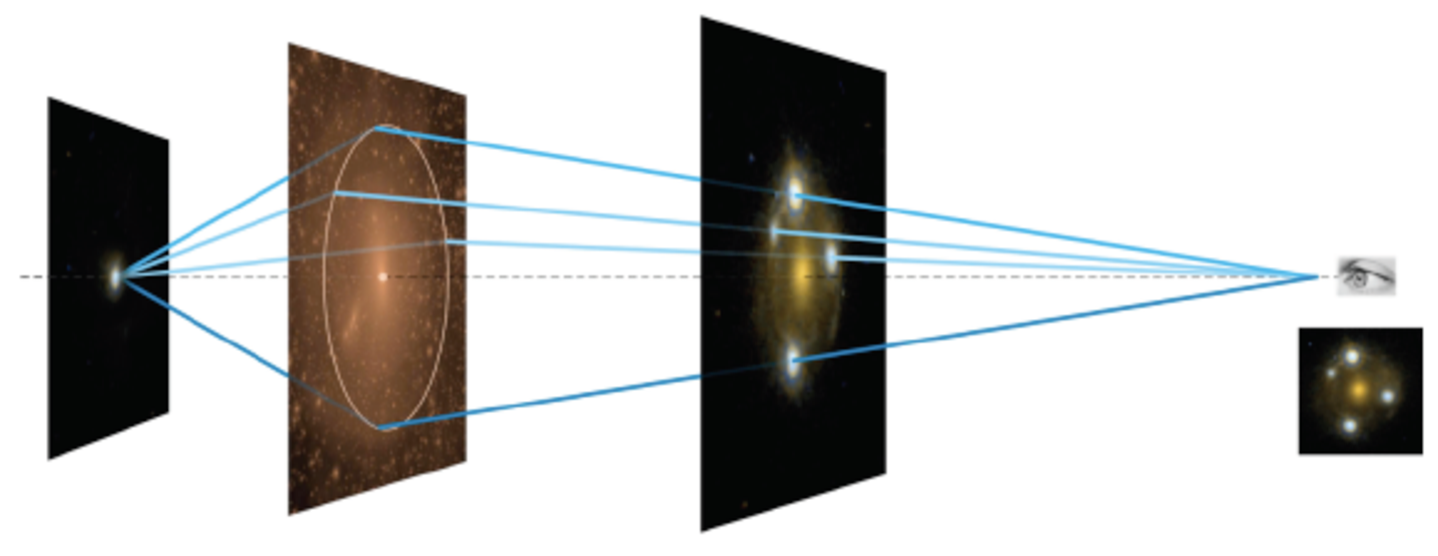
\includegraphics{raylensingdiagram.pdf}} 
  \figcaption{A cartoon of gravitational lensing. The source may be
    variable, resulting in fluctuations seen at different times at
    each image position. The lens itself may have a complex structure
    or environment.  \label{fig:ray}}
\end{center}
\end{inlinefigure}

Figure~\ref{fig:ray} illustrates the geometry of strong lensing. From
Equation~\ref{eq:arrivaltime}, we can intuit the main motivations for
measuring time delays to high precision.  The pre-factor is a
combination of angular diameter distances which are proportional to
$H_0^{-1}$, with a higher-order dependence on other cosmological
parameters. For example, Suyu+2013 reported on a a Hubble constant
measurement of $H_0=80.0^{+5.8}_{-5.7}$\,km\,s$^{-1}$\,Mpc$^{-1}$ from
time delay measurements of the four-image lens RXJ1131$-$1231 (Sluse
discovery paper) reported in Tewes2013 at a fractional uncertainty of
1.5\% (1$\sigma$), or an absolute uncertainty of $\sim1.6-2.1$\,days
(depending on the technique discussed).  An improvement in the time
delay precision with well controlled systematics has the potential of
translating to a corresponding improvement in the lensing-derived
value of Hubble's constant.

If the \emph{absolute} time delay precision can be pushed to the
levels of hours or minutes, then a completely new door can open.  One
quarter of the total mass/energy budget of the universe today is
comprised of exotic dark matter material that interacts
gravitationally with baryonic matter. As galaxies assemble and evolve,
the properties and evolution of their substructure depends on the
thermal and interaction properties of the particle (or particles) that
make up the dark matter. A robust census of substructure is a powerful
probe of the nature of dark matter itself. Strong gravitational
lensing is capable of measuring this substructure, and significant
advances have been made recently using combinations of lensing
observables. The observable that has been largely untapped for
substructure is the time delays between lensed images, because of the
level of precision that is required to provide comparable
constraints. Yet time delay constraints are highly desirable as they
are direct and proportional tracers of substructure perturbations in
the lensing potential, and are sensitive to very large projected areas
around lens images. As demonstrated in Keeton \& Moustakas (2009),
time delay perturbations from substructures with mass scales at or
below dwarf galaxies are on the order of one to a few hours, setting
the target precision necessary, to gain traction on the dark matter
substructure measurement.

The topology of the arrival time surface expressed in
Equation~\ref{eq:arrivaltime} gives further insight into how lensed
images form, and what the time-order sequence of the images is
expected to be. In particular, images will form at the critical points
of the time delay surface, and for an observed four-image lens
configuration, the leading image will be the first minimum (M1),
followed by the second minimum (M2), then the first saddle-point (S1),
the second saddle-point (S2), and finally the maximum point. Since the
maximum point of the surface is often heavily obscured by the lensing
object, in addition to being severely de-magnified, we ignore it and
concentrate on the four visible images.  For a time-varying lensed
source, a fluctuation is expected to be observed in the sequence
M1-M2-S1-S2 (Williams-Saha; Blandford), and we adopt the convention of
always correlating the measured light curve of a \emph{trailing} image
to that of a \emph{leading} object, so that in general, a positive
number may be expected. In cases where a negative delay is measured,
exciting insights may be possible through the challenge to the
assumptions used in building the basic lens model.  These may include
the effects of dark matter substructure, which can modify the
underlying projected potential near one or more of the formed images,
to the level of affecting the topology of the time delay surface
significantly (KM09).

In this work, we embark on a pilot ground-based experiment to explore
what absolute time delay precision may be possible, and what the
limitations and advantages are to pursuing this. As our target we
select one of the brightest four-image lensed quasars known to date,
HE0435$-$1223, which is additionally benign by having a relatively
faint lensing galaxy and uncomplicated environment.  We describe the
experimental design in Section~\ref{sec:design}, 

% Concept of PSF photometry. Advantages and cautions of the approach,
% compared to aperture or Kron photometry. Strengths in crowded fields
% where the PSF may be well determined.  

\section{Experimental Design\label{sec:design}}

Through the LCOGT peer review process, we were awarded a total of
180\,hours to pursue observing campaigns on two objects, HE0435 and
RXJ1131.  We planned on as optimal timing of the observations as was
possible.  With HE0435, we took a series of sample observations in
2014~October to test our planned integration times and our data
reduction pipeline, described below, and executed our campaign during
New Moon in 2014~December.  The observations of RXJ1131, planned for
New Moon in 2015~March were never possible to schedule, due to
technical issues. 
% \subsection{Motivation}
% 
% We were awarded 180\,hours of 1-meter time with LCOGT in Cycle 2014B,
% which were intended to be split between two targets, HE0436 and
% RXJ1131.  The latter observations were not possible as explained
% later, so the current work focuses on HE0435.  
% 
% Politics.  Keen on finding out what is the best possible time delay
% measurement that is possible from the ground with a dedicated
% project.  Also interested in stress-testing the LCOGT system, which is
% experience powerful for evaluating possible performance for other
% science applications.  
% 
% Add comment on how the original request and award included
% observations of RXJ1131, which were not possible in the end. 

\subsection{The Target, HE0435$-$1223}

\begin{inlinefigure}
\begin{center}
  \resizebox{\textwidth}{!}{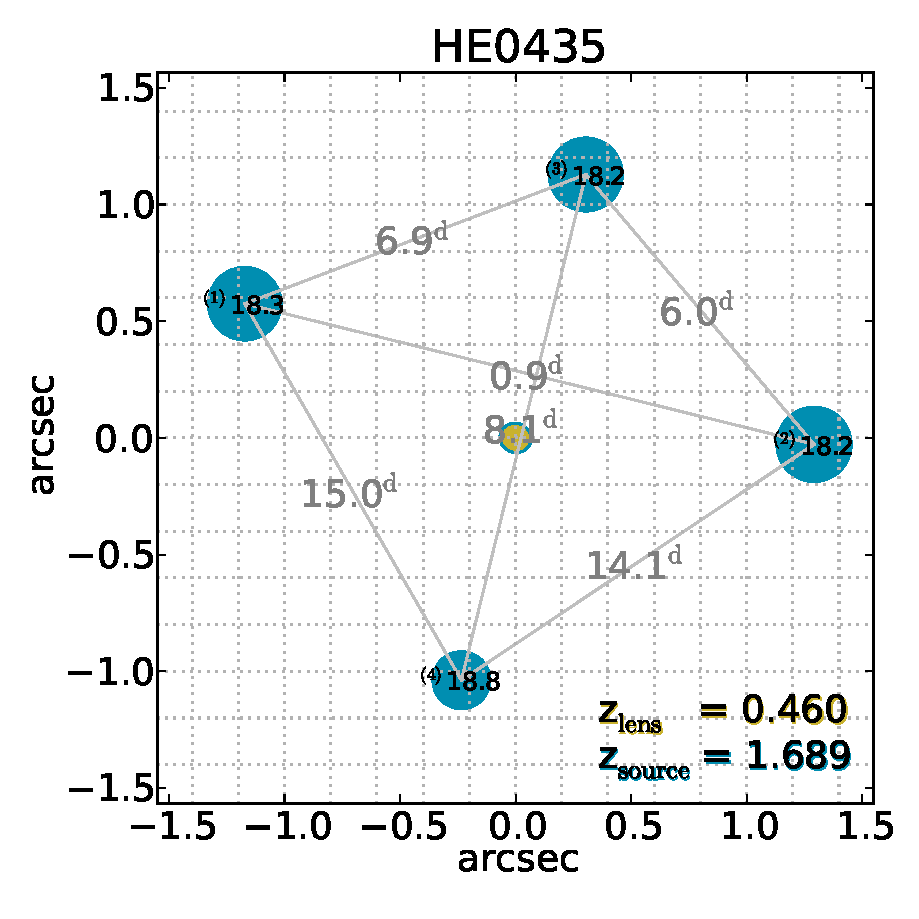
\includegraphics{HE0435.pdf}} 
  \resizebox{\textwidth}{!}{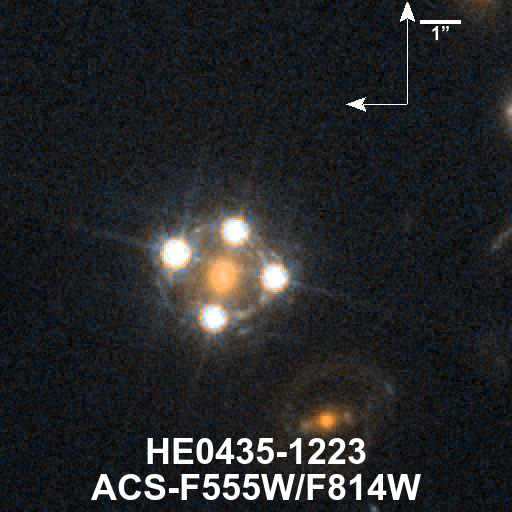
\includegraphics{HE0435-1223_ACS_F555WandF814W_ZOOM2.png}} 
  \figcaption{The target.}
\end{center}
\end{inlinefigure}

Figure of MLD cutout, with annotations.  Redshifts.  Estimated black
hole mass and luminosity, this connects to expectations for the
statistical behavior of its light curve, important later.  What general and
fun things are known for this system and its environment.  Time delays between
images. Pair that informed the conceptual design of our project.
Tirade on translation of stupid image naming to sensible topologically
motivated naming.  

Table, basic properties of target and relative positions of
images. This is the basis of the template of the ``system'' used in
the fits described later. 

This system is a quasar at $z_{\rm source}=1.689$ multiply-imaged by a
foreground massive galaxy at $z_{\rm lens}=0.460$ into a ``fold''
geometry.  

\input{phobi_he0435.tex}

\subsection{The Las Cumbres Observatory Global Telescope Network}

% What is LCOGT, Table of observatories in the network and the ones that
% we used, with their main properties. Aperture, field of view, pixel
% scale, gain, readnoise. 

The Las Cumbres Observatory Global Telescope (LCOGT) network is an
integrated system of telescopes located at excellent astronomical
sites around the world.  A technical description of the physical
components of the network is given in \citep{brown13}. The 1-meter
sub-network includes nine telescopes instrumented with optical imagers.
These telescopes are located at four sites, three in the southern
hemisphere (Chile, Australia, and South Africa), and one in the
northern hemisphere (Texas).  Observations are requested as one or
more consecutive exposures defined by a sky position, a filter, and an
exposure time during a time window.  A single software scheduler
assigns the observation to a particular telescopes which carries out
the observation robotically and returns the data to LCOGT
headquarters. There, the images are processed in order to remove
instrumental signature and made available to the user within a few
hours of the observation.

At the time of the observations presented here, the imagers on the
1-meter LCOGT telescopes were split between two types.  Two of the
telescopes in Chile were equipped with imagers, called "Sinistros",
based on Fairchild CCD486 detectors.  These are thinned,
back-illuminated 4096 X 4096 CCDs with 15 micron pixels, which produce
a 26.4 X 26.4 arcmin field of view with 0.39 arcsec pixels.  The
remaining telescopes were equipped with SBIG STX-16803 cameras, which
are based on Kodak KAF-16803 detectors.  These are unthinned,
front-illuminated 4096 X 4096 CCDs with 9 micron pixels, which produce
a 15.8 X 15.8 arcmin field of view with 0.23 arcsec pixels.  These
were operated in a 2 X 2 binned mode.  The Sinistros have typical read
noise of 10 electrons, while the SBIG imagers have typical read noise
of about 15 electrons.

Only telescopes at the three southern sites were used in this study,
and the parameters of the sites, telescopes, and instruments used are
summarized in Table x.

% \begin{thebibliography}{}
% \bibitem[Brown et al.(2013)]{brown13} Brown, T. et al. 2013, \pasp, 125, 1031
% \end{thebibliography}
\begin{deluxetable}{lcccc}
\tablenum{1}
\tablecaption{LCOGT 1-meter Telescopes used in this study }
\tablehead{\colhead{site} & \colhead{location} & \colhead{telescope} & \colhead{imager}  & \colhead{imager type}}
\startdata
LSC & CTIO, Chile & 1m0-04 & fl04 & Sinistro\\
LSC & CTIO, Chile & 1m0-09 & fl03 & Sinistro\\
COJ & Siding Spring, Australia & 1m0-03 & kb71 & SBIG STX-16803\\
CPT & Sutherland, South Africa & 1m0-10 & kb70 & SBIG STX-16803\\
\enddata
\end{deluxetable}

\section{The Observations}

\subsection{General Description}

Using the Las Cumbres Observatory Global Telescope (LCOGT) Network
\citep{Brown13}, we (nearly) continuously monitored the
gravitationally lensed quasar HE0435-1223 \citep{Wisotzki02} for
$\sim 50$\,hours. Our observations used the 1-meter class telescopes in
Australia, South Africa, and Chile. The Sinistro camera was used in
Chile, but was not available in South Africa or Austrailia, so the
SBIG cameras were used at these sites instead. Our observations were
taken from 2014-12-16 to 2014-12-18, corresponding to approximatly new
moon limiting sky brightness contaminiation.
	
Each exposure was $300$\,s, which yields good signal-to-noise for a
source at $r = 19.5$, approximately the brightness of the lensed
images, but short enough to measure time delays to high precision. The
primary campaign was completed in $r$-band, but 6 $g$-band exposures
were taken intersperced throughout the night to control for color
variation.
	
Across $\sim 50$\,hours, we lost one night in Australia to bad
weather. Most of the good weather data was taken successfully, but a
few frames were adversely affected by shutter failures. These frames
were rejected by eye and will not be considered in the subsequent
analysis. Our final dataset includes 385 images taken over
$\sim 50$\,hours, with a total integration time on the target of
$32$\,hours \textbf{We need to check the numbers to make sure these
  are what Andrew used.}.
	
\begin{inlinefigure}
\begin{center}
  \resizebox{\textwidth}{!}{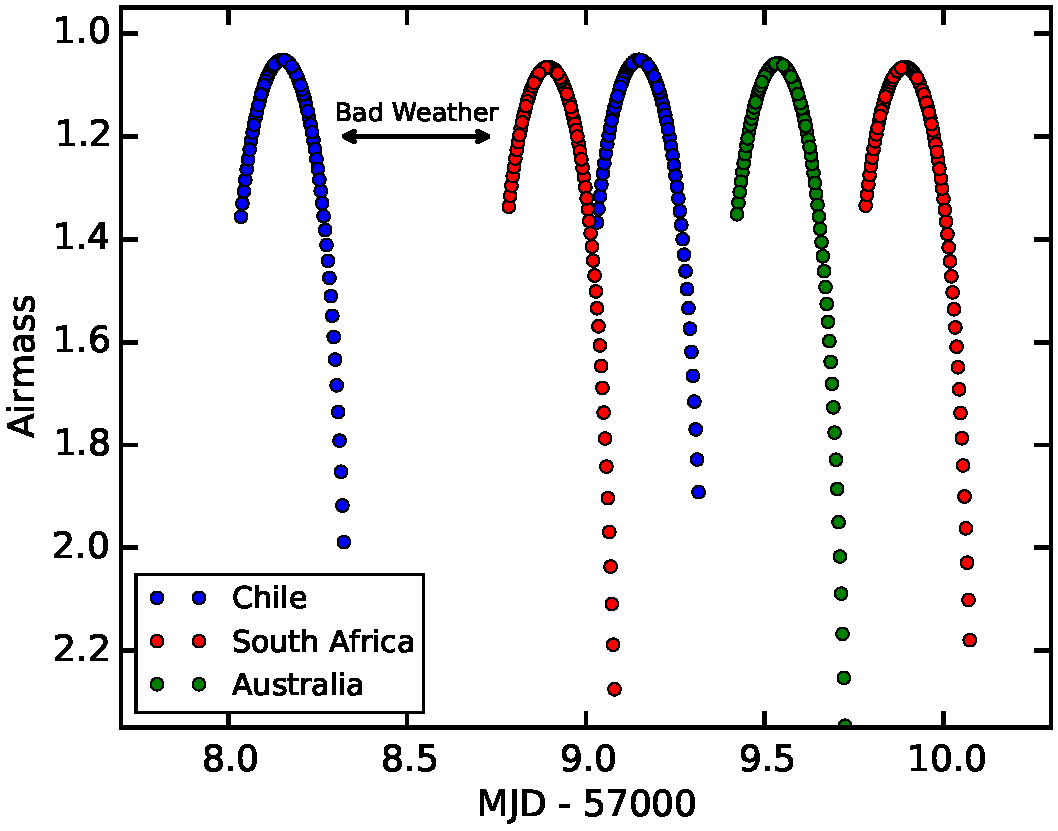
\includegraphics{he0435_airmass.pdf}}
  \figcaption{Airmass versus time for the actual sequence of
    observations of our HE0435 target, across all LCOGT observatories
    used. }
\end{center}
\end{inlinefigure}

% Figure of sky rms versus time.  Weather gap comment, which observatory
% and conditions. Shutter issue. High sky/background in some
% images, not fully diagnosed.  In the end, the data quality validation
% resulted in a sequence of XXXX frames, each with an integration of Y
% contiguously observed over Z hours of W days.  

\subsection{Data Reduction}
% Pre-processing, WCS correction, flatfields, cosmic ray identification
% and masking.  CCD counts gain-corrected before independently
% estimating readnoise. For COJ and CPT, readnoise estimated at
% 25\,counts.  FIGURE of ReadNoise by Observation, slide 11 of 0325
% presentation.  Reduction, APASS stars, zeropoint calculations and
% estimated robustness and uncertainty in zeropoint, PSF models with
% circular Moffat empirical model, fitting alpha and beta parameters.
 
The instrument signature was removed from the LCOGT images using
standard techniques, using a custom pipeline written in Python. For
each night/telescope, full frame bias and darks were median stacked
and subtracted from each science frame. The data were flat fielded
using median stacked twilight sky flats, taken within a few days of
our obsevations. Flat fields for any given filter are taken on a
rotating basis at each LCOGT site, so same-night flat field frames
were not always available. The astrometric world coordinate system
(WCS) was calibrated using Astrometry.net \citep{Lang10}. Cosmic rays
were identified using a modified version of the LA-Cosmic algorithm
\footnote{\url{https://github.com/astropy/astroscrappy})}
\citep{vanDokkum01}.
	
The read noise was estimated for each image by examining a series of
31$\times$31 pixel cutouts of the image. The noise is approximately
the poisson contribution from the sky photons and the read noise (we
include all non-poisson contributions, e.g. dark current, as ``read
noise''). We fit a Gaussian to the brightness distribution of each of
the 1000 cutouts, and then take the median of the standard deviations
to obtain an estimate of the read noise. We find that the SBIG images
have a read noise of $\sim 25 e^{-}$ and the Sinstro frames have a
read noise of $\sim 10 e^{-}$.
	
% APASS catalog used, 29 isolated stars used for calibration, spanning
% $r_{\rm SDSS}=14.2..16.5$ and $g_{\rm SDSS}=14.6..16.8$.   The
% photometric uncertainty for each reference star is
% $\approx0.03-0.10$\,mag, and as an ensemble the photometric zeropoint
% is determined to $\sim0.01$\,mag in the mean, whereas the weighted
% rms is $\sim0.02..0.04$.  
 
The zeropoint of each image was calibrated to the AAVSO Photometric
All-Sky Survey (APASS) catalog. A set of 29 isolated stars spanning
$r_{\rm{SDSS}} =14.2..16.5$ and $g_{\rm{SDSS}} = 14.6..16.8$ were
chosen to use for the zero point calibration.  The catalog uncertainty
for each individual reference star is $0.03-0.10$ mag, yielding a
final precision of $\sim 0.01$ mag.
	
%In future work we will present a fully self-contained Bayesian
%inference analysis suite, but for the present hybrid
%frequentist/bayesian approach there is a question of how properly to
%propagate zeropoint uncertainties, i.e.\ uncertainty in the mean, or
%the weighted rms.  
%[Equations if we want to].  

% How observations were set up and planned. Integration time
% calculations.  Two bands. Main campaign in one band, supplemented by
% second, for including color terms. [Question, we have ignored color
% terms in the present analysis, right? Is there a simple way of
% including this information in the calibraion and analysis that
% follows?] 

% The cadence and total campaign length of observations.
% Figure of visibility of target for our dates of observation, across
% network's observatories.  We observed through new moon.  Generally, we
% optimized the conditions for the observations in terms of phase of
% moon and visibility of the target as much as possible.  

% \begin{inlinefigure}
% \begin{center}
%   \resizebox{\textwidth}{!}{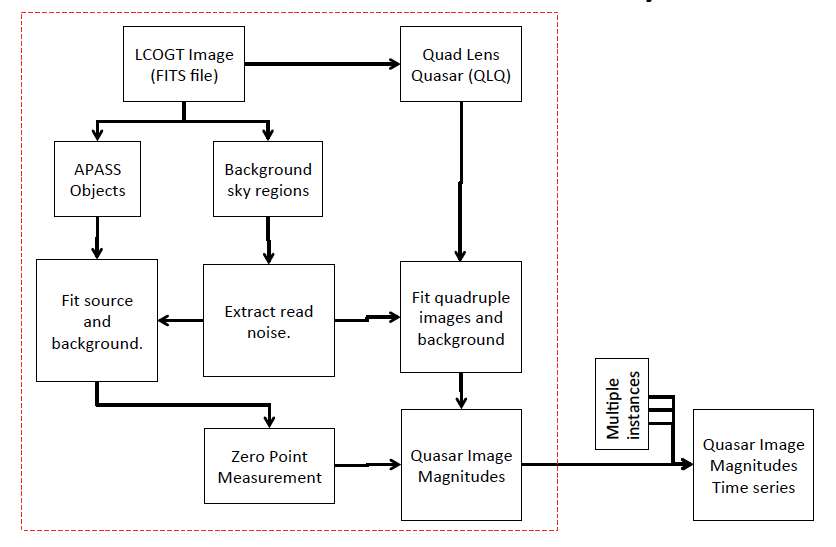
\includegraphics{LCOprocessdiagram.png}}
%   \figcaption{General procedure adopted. }
% \end{center}
% \end{inlinefigure}

\section{Analysis and Results}

\subsection{PSF Photometry of Target and Light Curves}

The point spread function (PSF) of the image was determined by fitting
a circular Moffat profile,
\begin{equation}
f(r) = \frac{2 r (\beta - 1)}{\alpha^2} \left[ 1 + \frac{r^2}{\alpha^2}\right]^{-\beta}
\end{equation} to the APASS stars, fitting for seeing parameters $\alpha$ and $\beta$.
	
The photometry of the lensed quasar images was derived using PSF
photometry. The seeing parameters were fixed from the APASS stars that
were used to determine the zeropoint. The quasar separations were set
to the positions from \citet{Courbin11}. The lens galaxy is faint in
the optical bands so its contribution is considered to be
negligible. The center of the lens ``system'' and the brightness of
each lensed image were allowed to vary in our fits for each
observation.  The final posterior distributions of fluxes and for each
of the lensed images were derived using the MCMC package emcee
\citep{ForemanMackey13}.

The full width at half maximum (FWHM) is 
\begin{equation}
{\rm FWHM}=2\alpha\sqrt{2^{1/\beta}-1}. 
\end{equation}

\begin{inlinefigure}
\begin{center}
  \resizebox{\textwidth}{!}{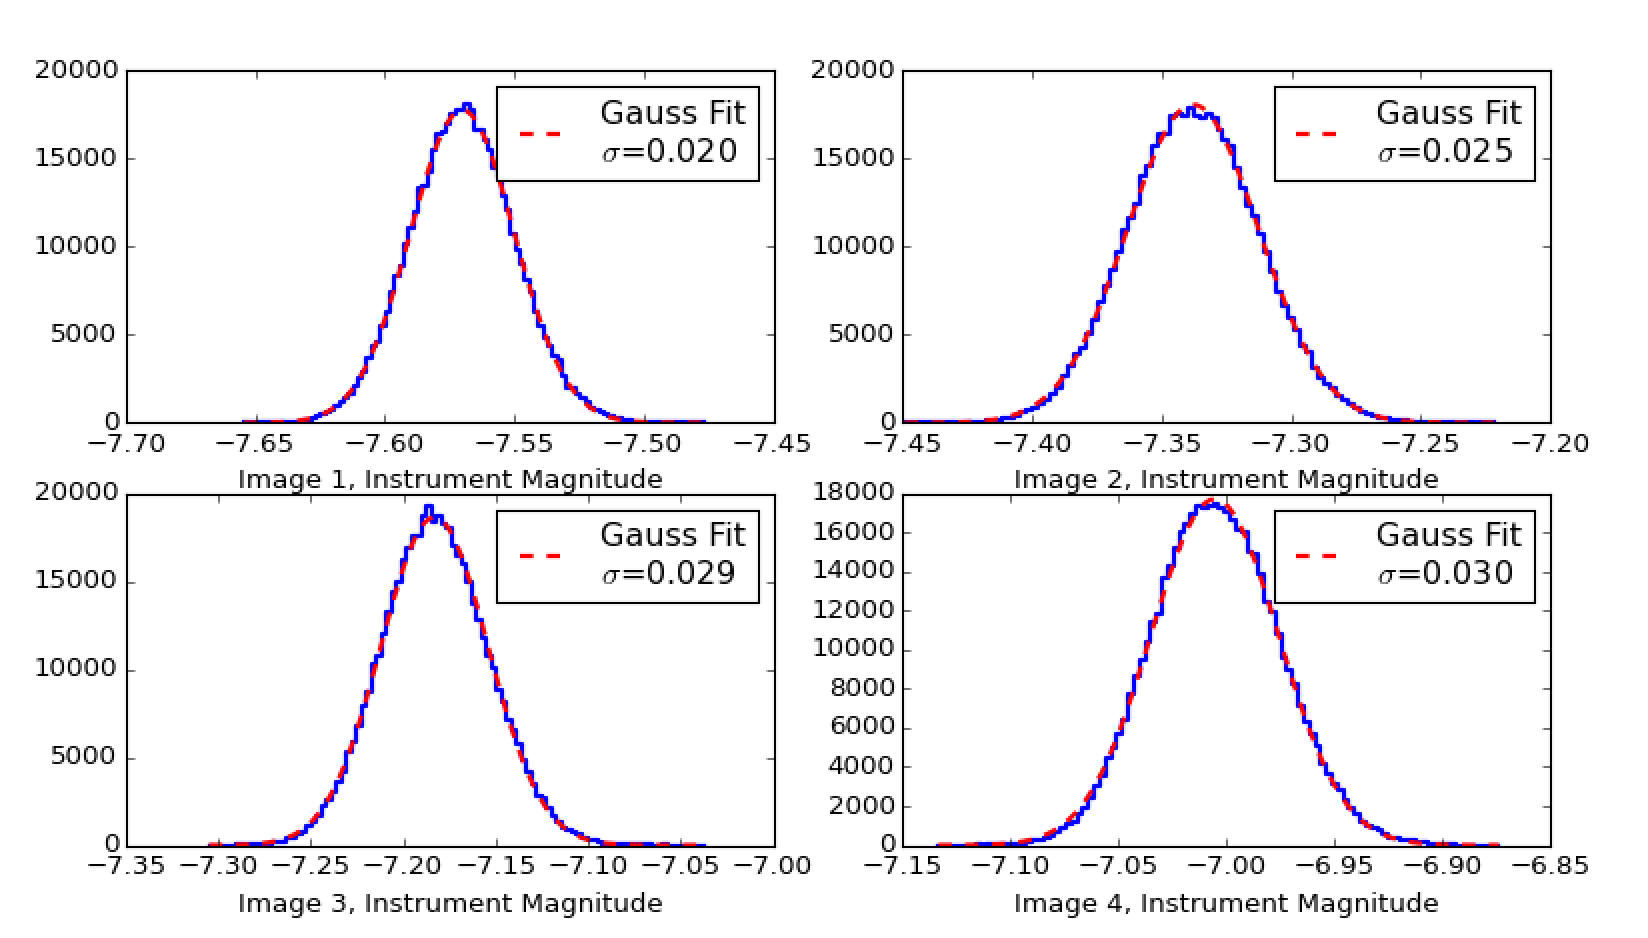
\includegraphics{instrumentalphotometrydemo.png}}
  \figcaption{Demonstration of the photometric measurement of each of
    the four quasar images, marginalized over the remaining parameters
    of the fit.  }
\end{center}
\end{inlinefigure}

Inference process setup for PSF photometry. Bayes' equation and model
setup.  emcee. Prior ranges. Numbers of walkers. Keep this very
simple. Demonstration of example triangle plot from photometric fit.
Quote basic representative numbers for photometry of images.  Lead-in
to FIGURE of killer figure, of propagated uncertainty versus time for
all images. 

\begin{inlinefigure}
\begin{center}
  \resizebox{\textwidth}{!}{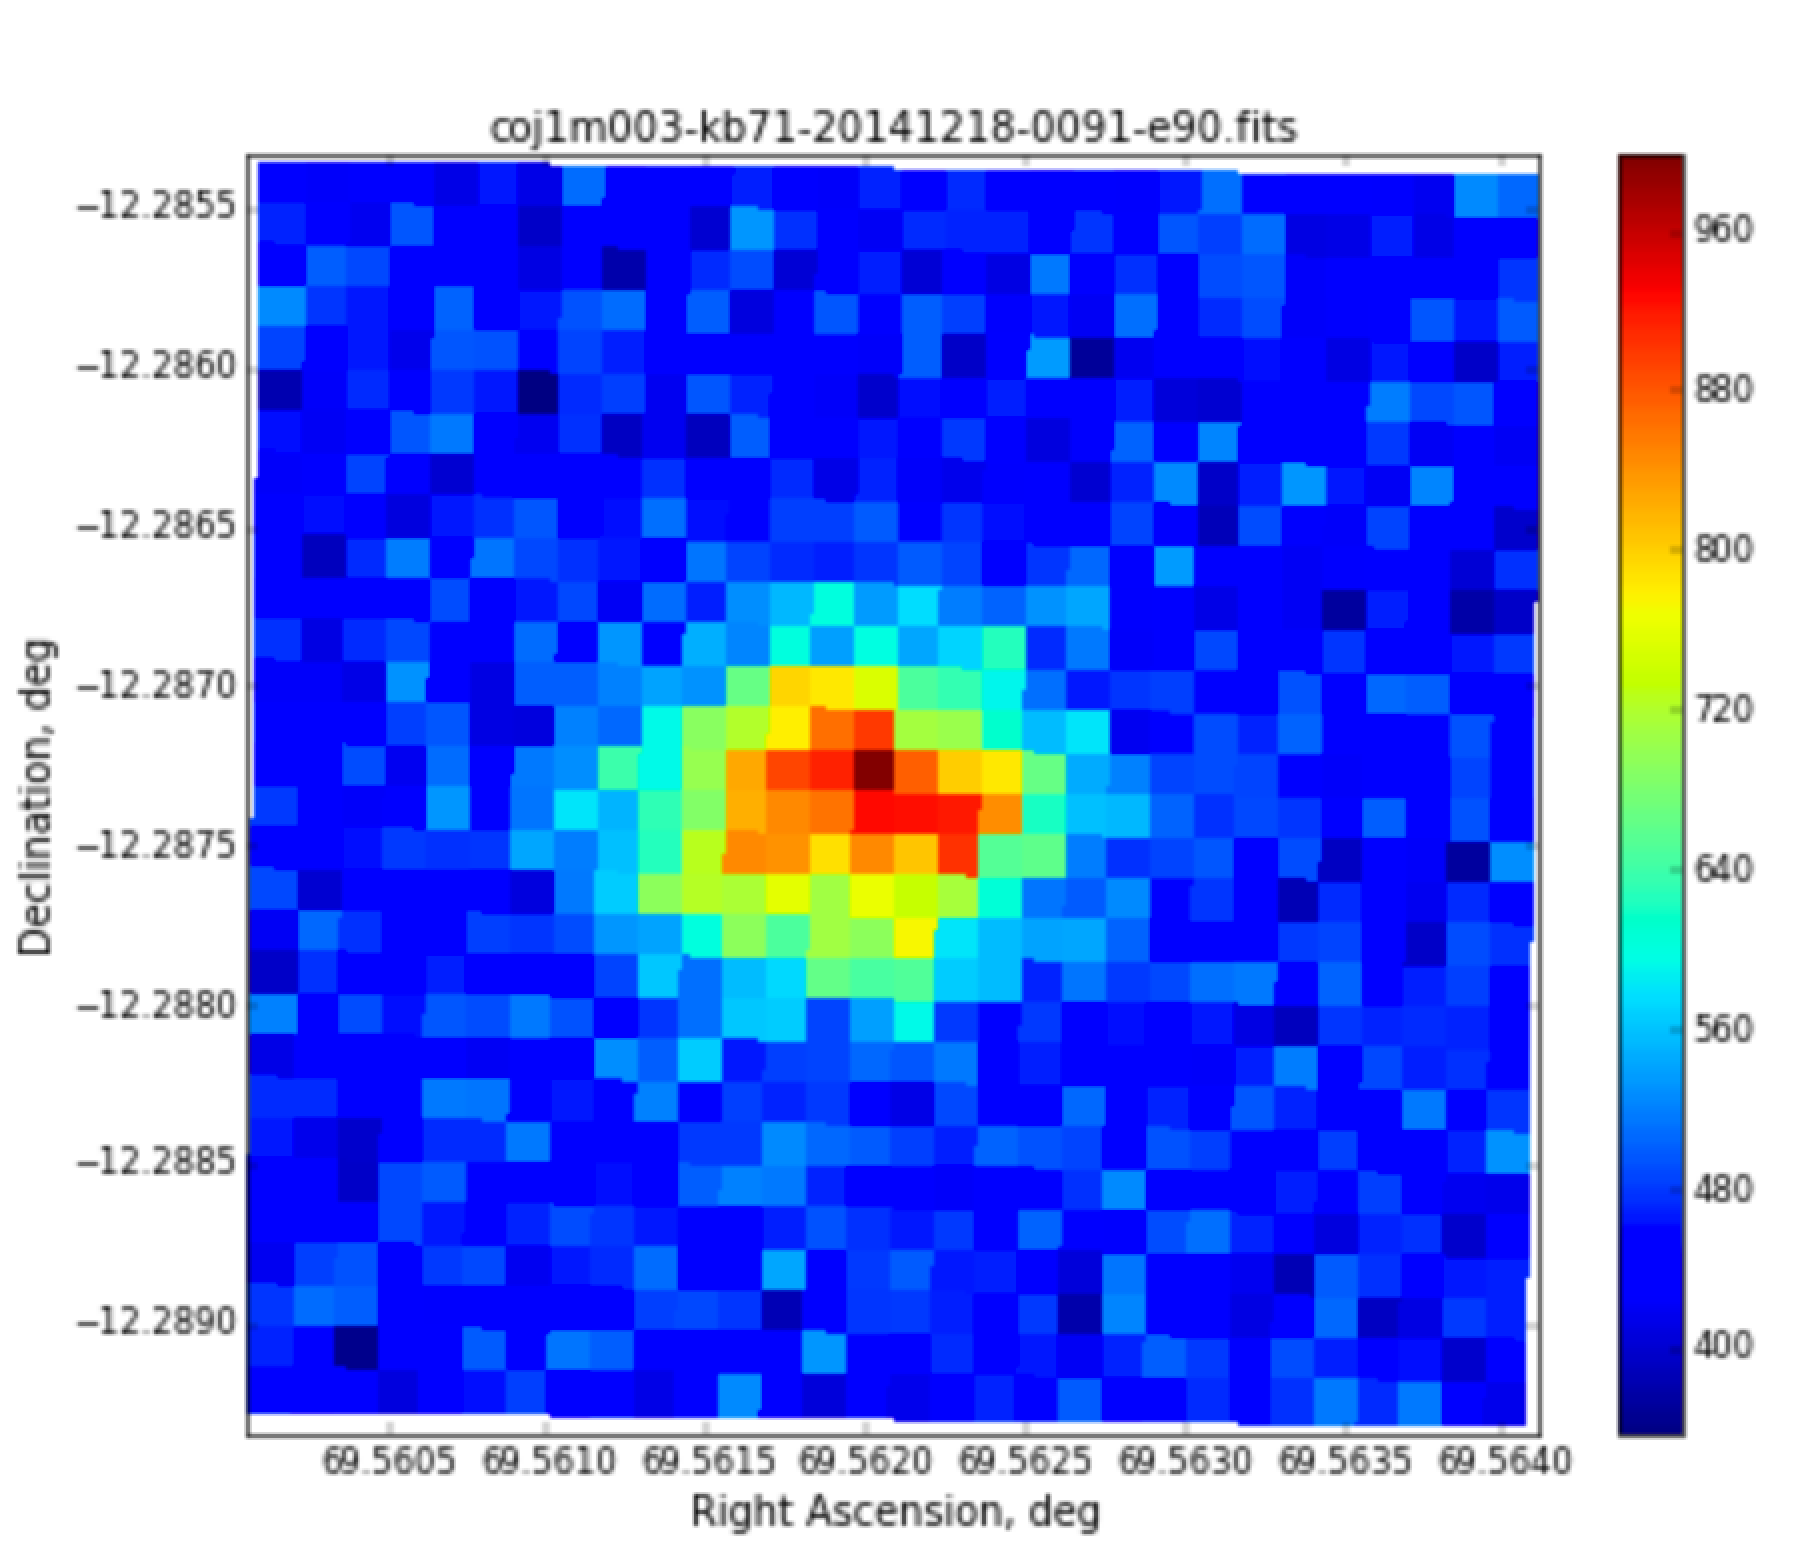
\includegraphics{samplelcogtimage.png}}
  \resizebox{\textwidth}{!}{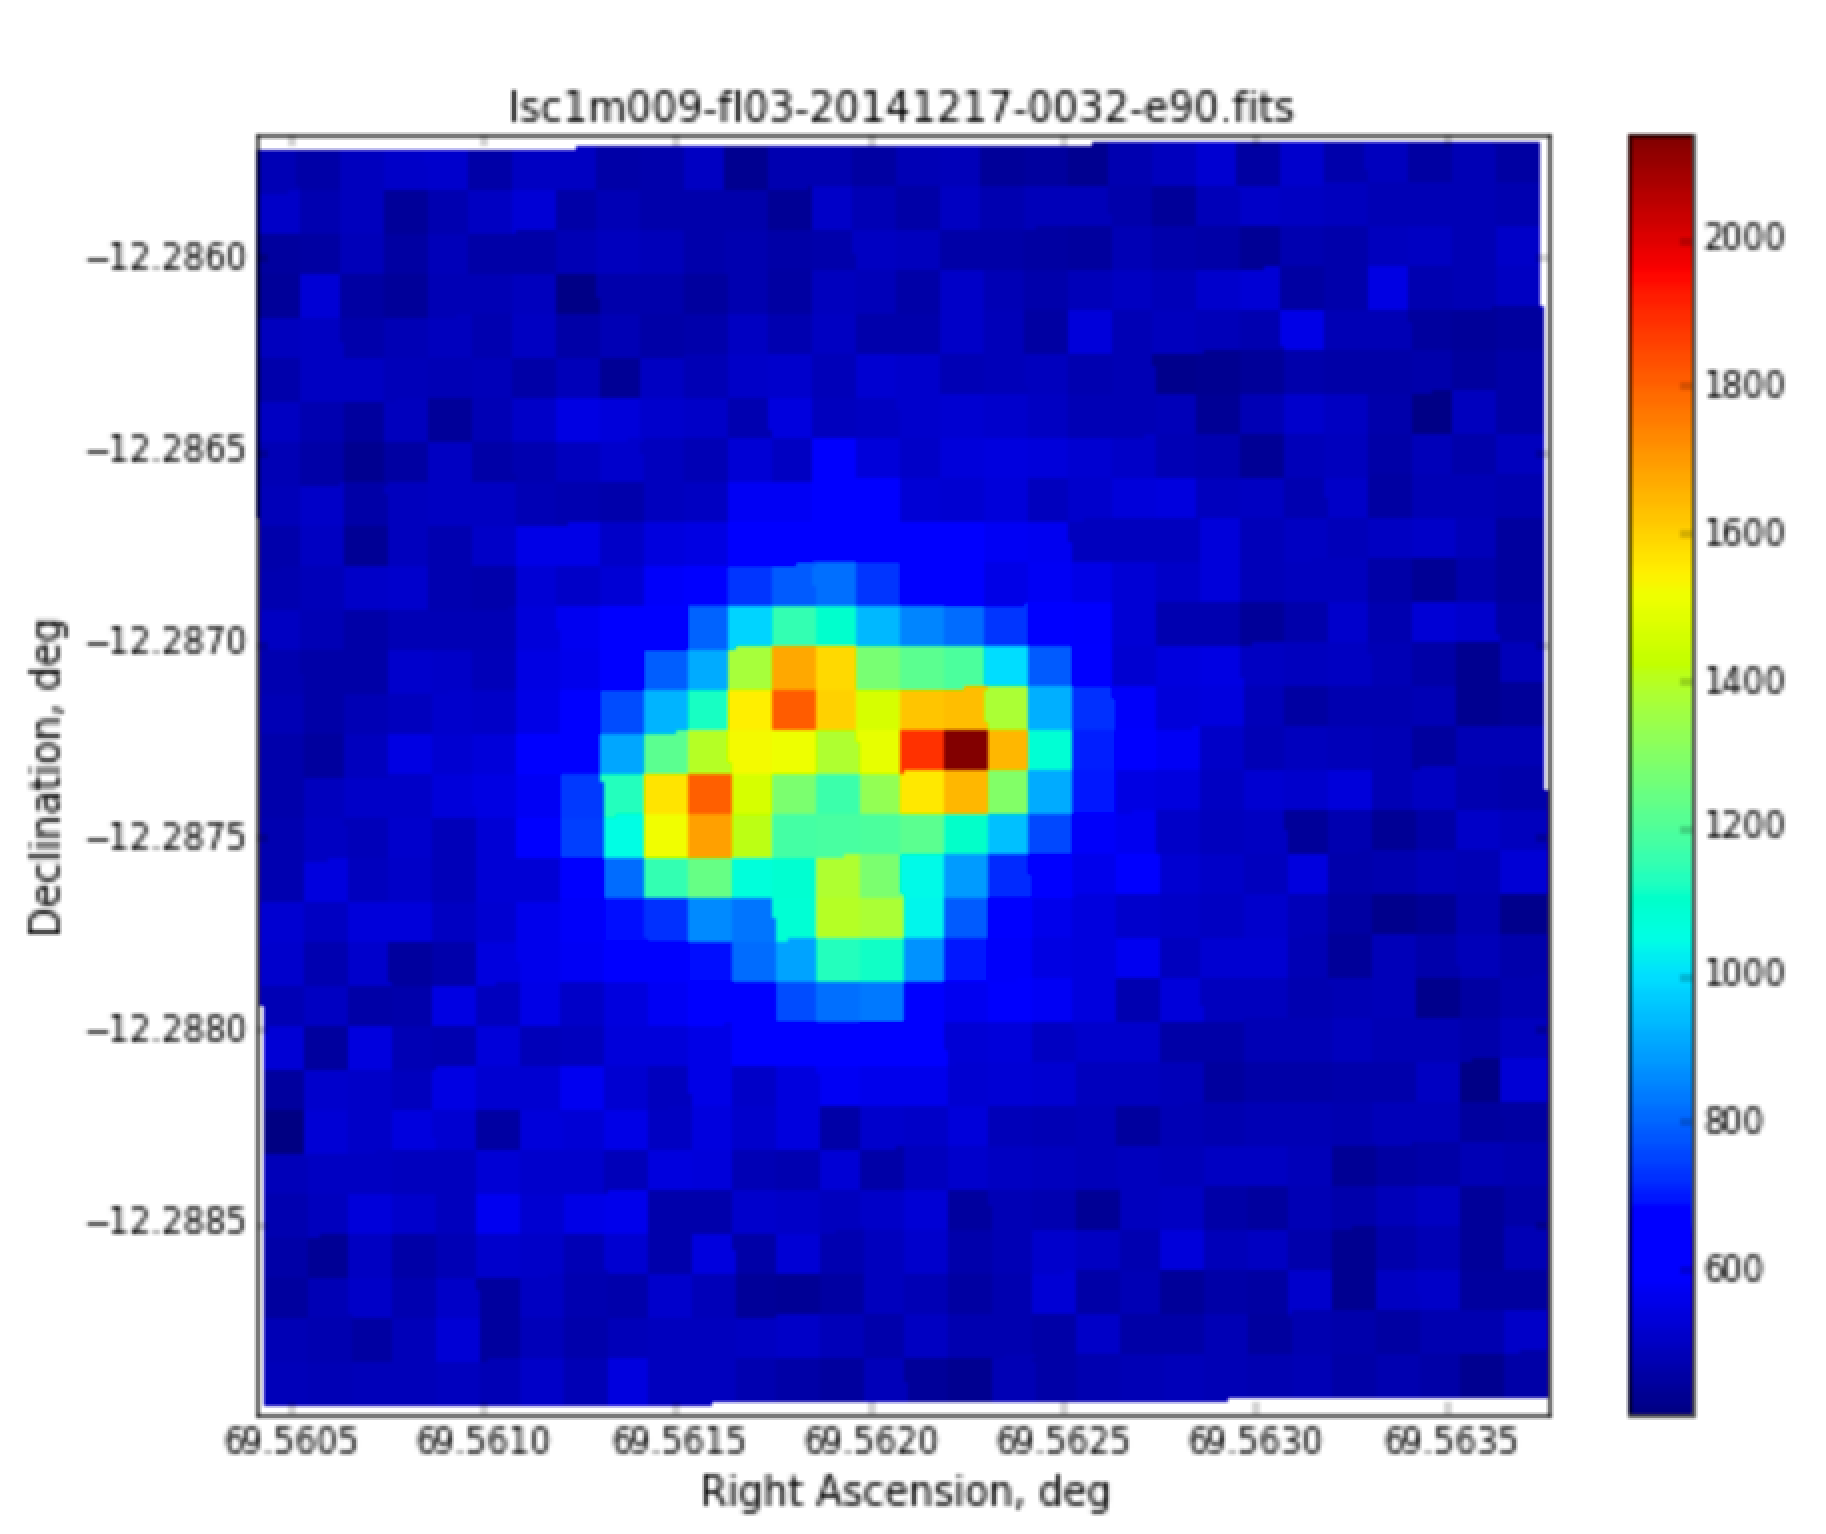
\includegraphics{prettygoodlcogtimage.png}}
  \figcaption{Two examples of observations, the first is a typical
    one, the second is one of the best ones. }
\end{center}
\end{inlinefigure}

\begin{inlinefigure}
\begin{center}
  \resizebox{\textwidth}{!}{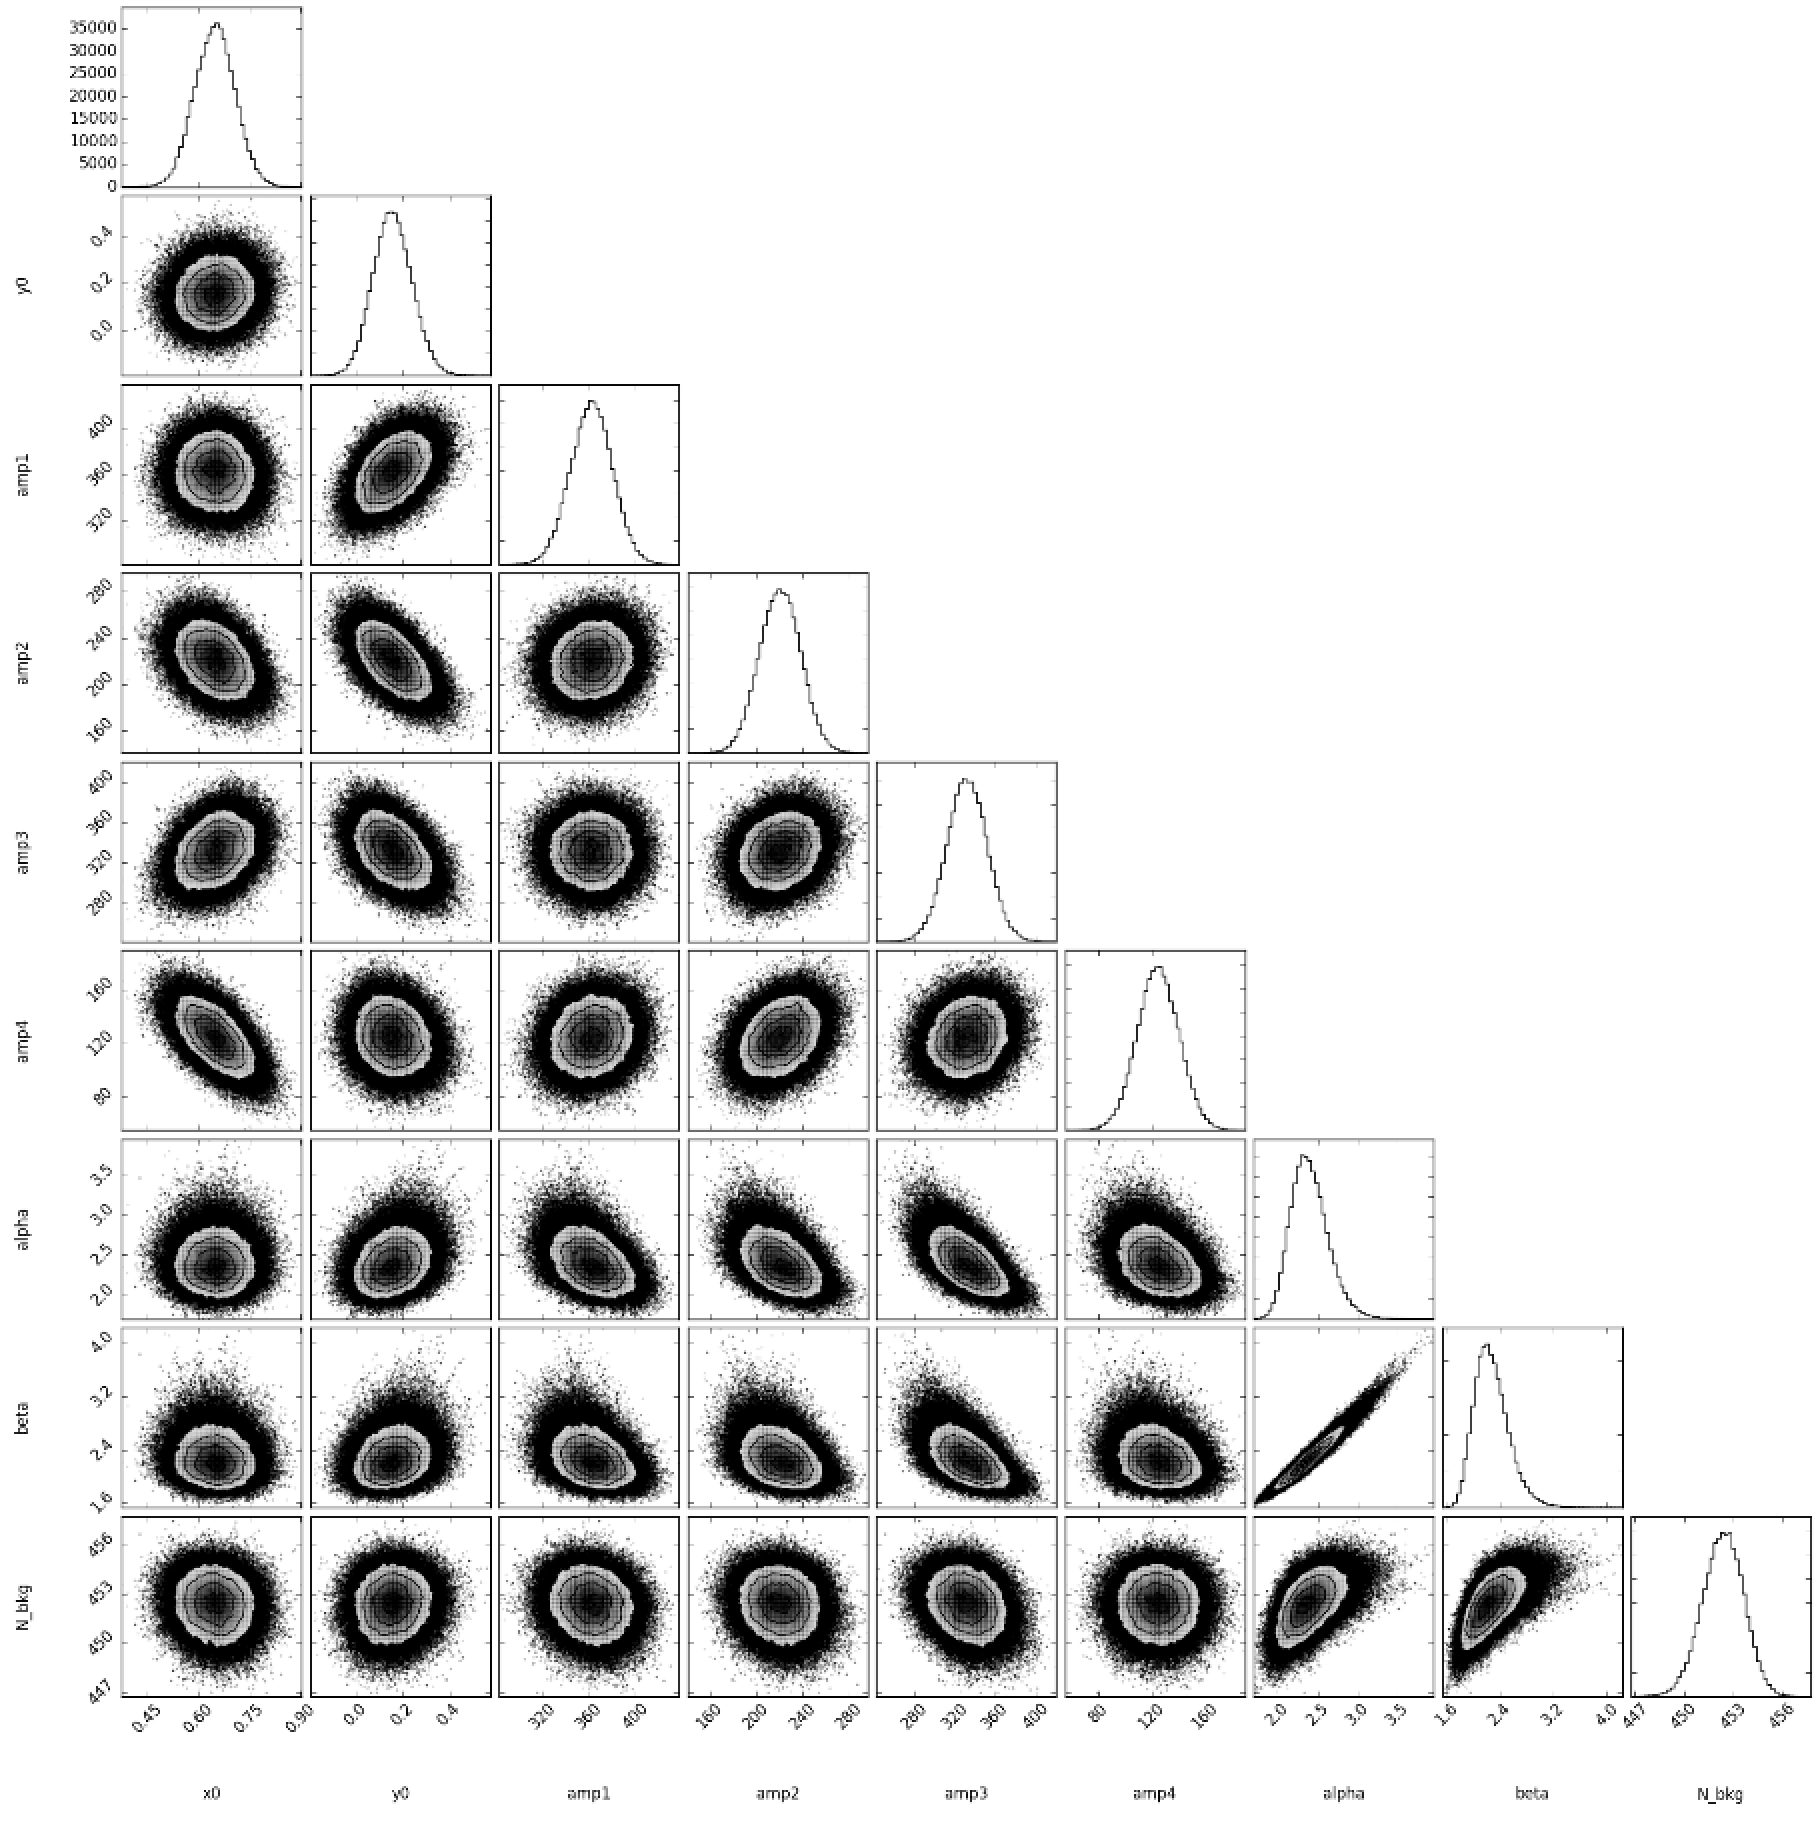
\includegraphics{samplephotinferencefit.png}}
  \figcaption{A demonstration of the results from inference on the
    four-image lens system, showing the ``system'' position ($x_0$ and
    $y_0$), the measured photometry in each of the four images, the
    adjusted parameters of the Moffat PSF ($\alpha$, $\beta$), and
    finally a fit to the local background flux level. }
\end{center}
\end{inlinefigure}

We show the instrumental flux measurements in the next figure, i.e.\
before calibration through the magnitude zeropoints, to illustrate the
differences across observatories, and that there are sections of
observations with observing overlap.  The final light curves after
calibration show consistency.  {\bf Actually, Andrew and all, let's
  dig into this a little bit more.  Particulalry for Image 3, is there
  a bit of a jump between calibrated observatories' measurements?. For
  images 1 and 2, there are 2-3 datapoints that look a bit odd or
  bumped up, through the rest look like reasonably okay overlap.
  Image 4 looks like a clean segue. Is that fair?  Do we have a
  systematic calibration effect to take into account?  Do we need to
  include a color-correction term, or fully remove the very
  high-airmass points? }
\begin{inlinefigure}
\begin{center}
  \resizebox{\textwidth}{!}{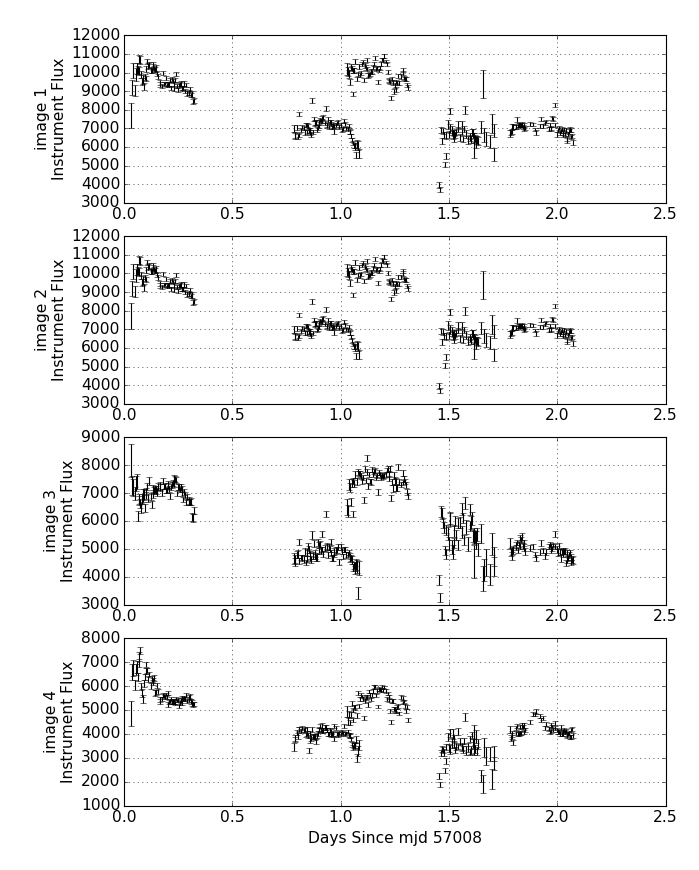
\includegraphics{instrumentalfluxes.png}}
  \figcaption{Light curves of observations for each lensed image. }
\end{center}
\end{inlinefigure}

This process is repeated across all vetted observations (of the band
we have concentrated on), to produce the calibrated light curves shown
in FIGURE for each lensed image.  
\begin{inlinefigure}
\begin{center}
  \resizebox{\textwidth}{!}{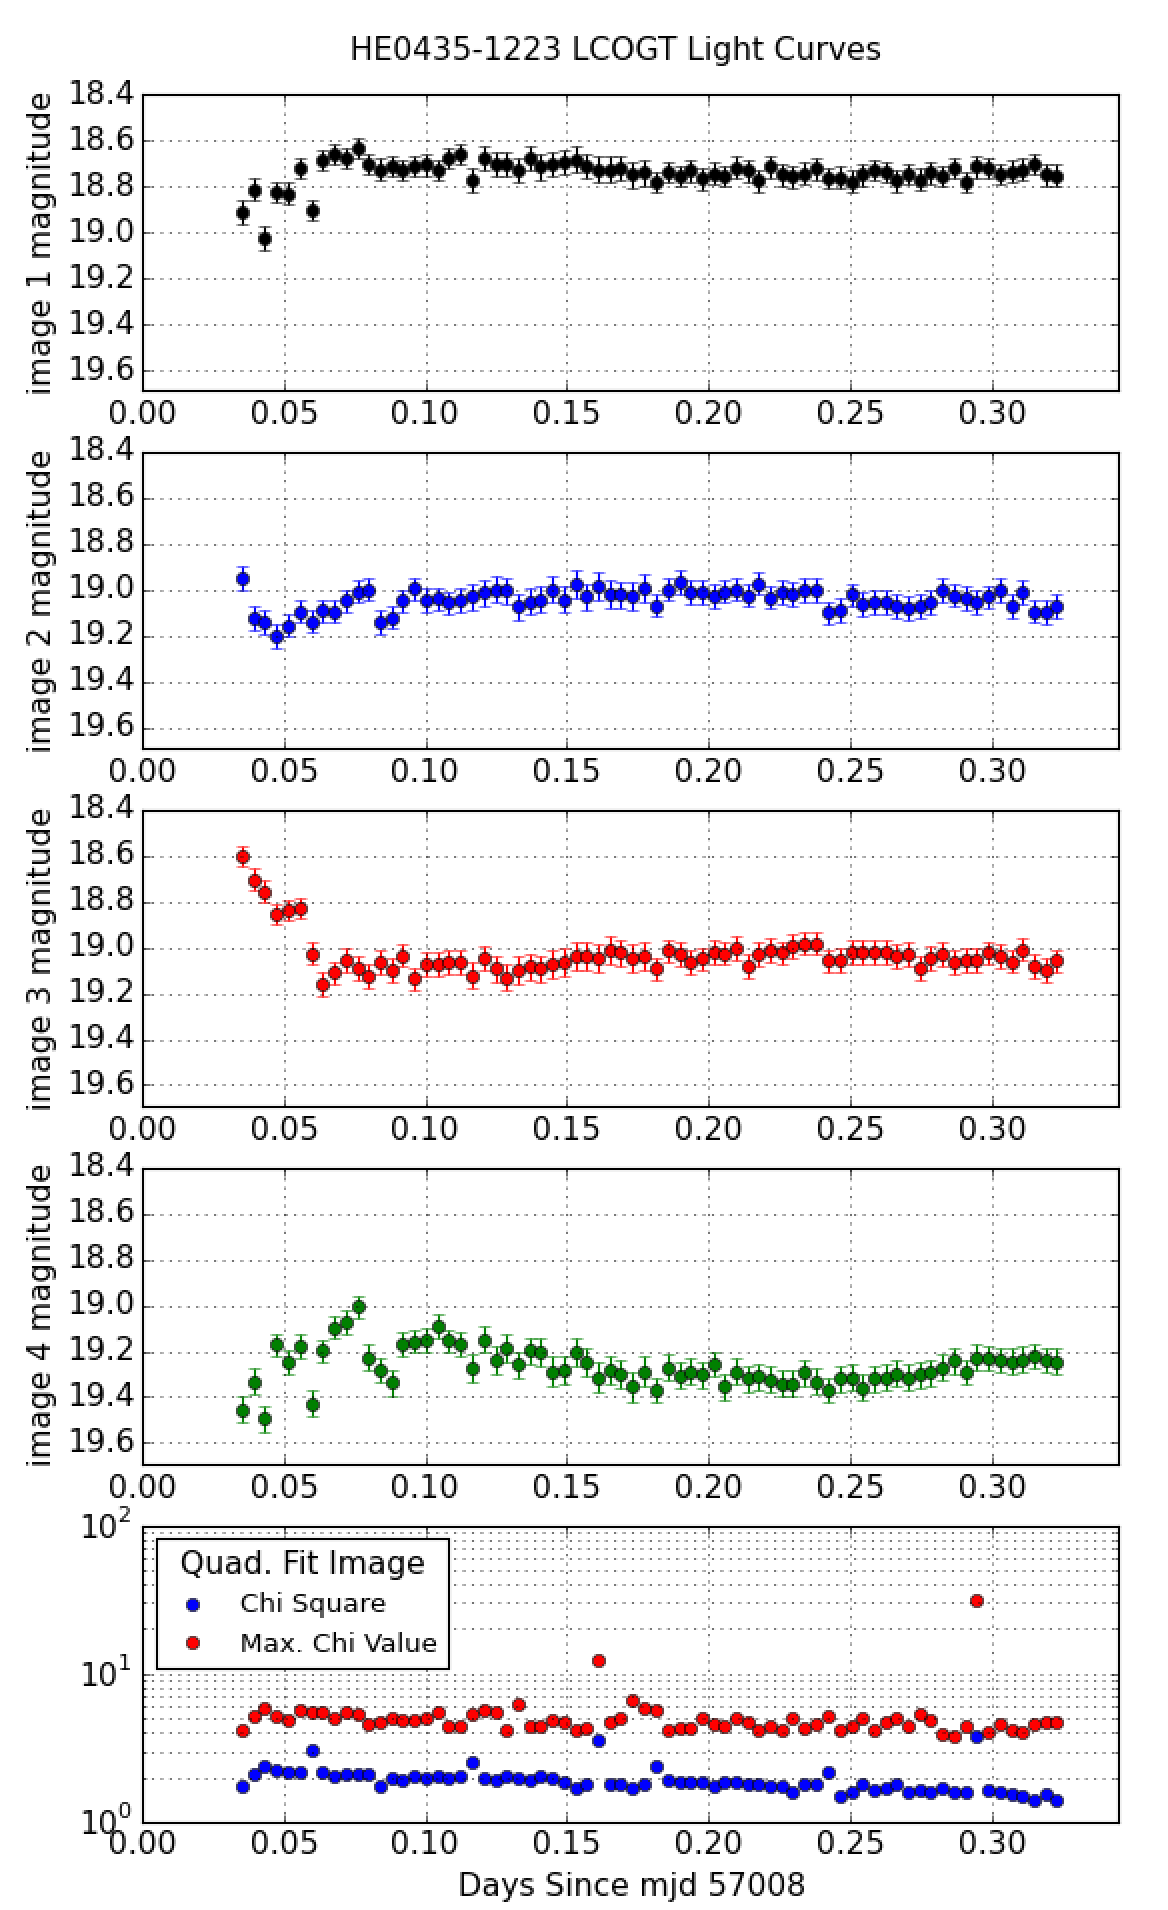
\includegraphics{firstlightcurves.png}}
  \figcaption{Light curves of observations for each lensed image. }
\end{center}
\end{inlinefigure}

A practical driver of this work is to empirically determine how the
photometric stability in an effectively ``crowded'' target field
behaves, and what the main sources of uncertainty are.  This
uncertainty budget and behavior is mapped in FIGURE.  
\begin{inlinefigure}
\begin{center}
  \resizebox{\textwidth}{!}{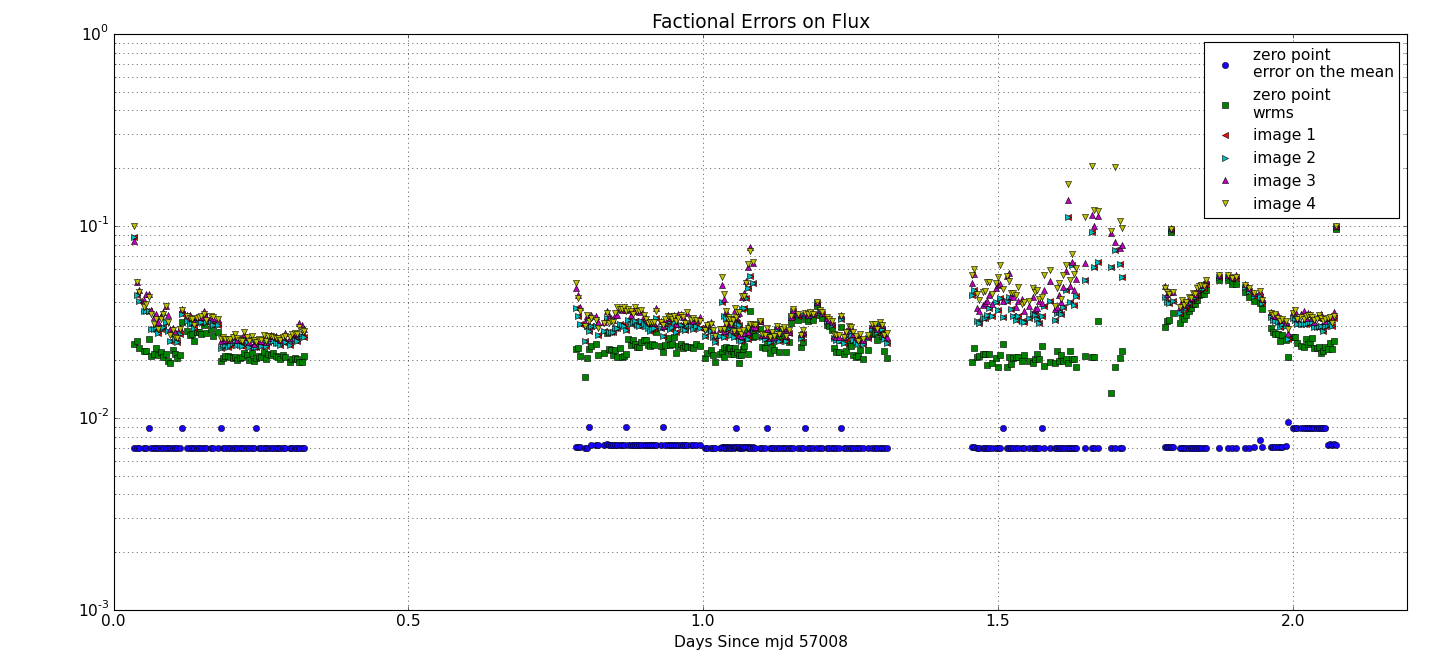
\includegraphics{fractionaluncertainties.png}}
  \figcaption{Summary of the fractional uncertainties in flux
    measurements for each lensed image, as well as the zeropoint
    correction uncertainties which formally are propagated to the
    total photometric uncertainties.  }
\end{center}
\end{inlinefigure}

\section{Time Delay Inference}

High level FOT and TDC review/recap, DRW motivation and method,
connection to black hole mass and luminosity. Structural tau sigma and
magnitude parameters that describe this gaussian process (refer to
relevant book) reasonably.  While we are ultimately interested in a
more fundamental understanding of how the quasar black hole accretion
physics maps to the optical light curve behaviors, we simply adopt
this parametrization presently.  

We also ignore microlensing, because of the short timescale of the
observations compared to the typical microlensing timescales (refer to
GERLUMPH as well as COSMOGRAIL).  

Bayes' setup for this case. Discussion of priors. Again using
emcee. Briefly on walkers etc setup.  

FIGURE triangle plot on the inference on light curve structural
parameters as well as time delays between different images' light
curves.  Sets of paired light curves, emphasis on AC.  General and
``ignorant'' exploration of behaviors, partly as a learning experience
with such data.  Also examined other pairings, even though based on
both models (Oguri reference?!) and cosmograil results from 7 years of
observations, expected to be longer.  

We also extract the ``time delay corrected'' baseline flux ratios,
which of course are not directly translatable to magnification ratios,
since microlensing differential magnification can be of order unity.
(Reference to gerlumph's estimated numbers, possibly adopt a figure
from them or at least quote ranges of numbers).  

Tabulate all results, vis a vis all other published data.  

Comment on exciting precision.  We have measured a 0.25-day time delay
to a precision of 30 minutes. 

\section{Discussion and Conclusions}

Discussion of found time delays versus cosmograil's, as well as
theory.  How these measurements are useful for H0 and cosmography.
Back of envelope calculation showing potential improvement with a full
model along the lines of Suyu?  Or use a Coe-Moustakas type estimator?  

Acknowledge importance of color-dependent microlensing as probe of
inner structure of black hole accretion disks, and how exciting that
is.  To extract high fidelity microlensing time behaviors, in effect
two light curves need to be subtracted off from each other, so that
the residuals can be examined.  Therefore, a robust time delay
improves this.  

Importance of this style or type of campaign.  High cadences are key
to high precision.  The photometric precision resulting from unstable
psf and highly varying background is very risky and dependent on the
fluctuation properties the quasar on the relevant timescales.  The
results here give a valuable insight into this.  Parallel work in
studying Kepler AGN light curves by several groups (Matt Malkan etc
etc etc, but also us) will lend more insight into this in the near
future.  

Ground versus space. Ground observations have a very clear and
powerful role to play.  Stress-testing of observations is a
challenge.  Advantages of a space-based platform improves and
guarantees performance on a host of areas [listed and quantified].  

\acknowledgements

This research was carried out in part at the Jet Propulsion
Laboratory, California Institute of Technology, under a contract with
the National Aeronautics and Space Administration.  This research was
made possible through the use of the AAVSO Photometric All-Sky Survey
(APASS), funded by the Robert Martin Ayers Sciences Fund.  Copyright
2015. All rights reserved.

\bibliographystyle{apj}

\bibliography{/Users/leonidas/Dropbox/bibdesk/moustakasbibs}
\bibliography{lcolens_datareduction}

\end{document}

% %%%%%%%%%%%%%%%%%%%%%%%%%%%%%%%%%%%%%%%%%%%%
% \section{Introduction}
% \label{Introduction}
% 
% Dark matter is an exotic, as yet undetected particle that, in enormous
% numbers, dominates the gravitational component of the universe. On
% astronomical scales, we can infer key facets of the nature of the dark
% matter particle through the study of strong gravitational lenses.
% Gravitational lenses are objects that are sufficiently massive and
% concentrated, that light from more distant luminous objects ends up
% forming multiple images. If the background, lensed object is changing
% its brightness with time, each brightness variation will be seen at
% different times at each of the images!  Measuring these "time delays"
% very precisely is potentially very powerful for inferring dark matter
% properties.  Actually measuring time delays involves making many
% independent measurements of a gravitational lens, obtaining a
% time-series for each image and estimating the time offsets between the
% observed light curves.  Acquiring such data requires many real
% astronomical images, making challenging photometric measurements with
% various approaches, and calculating light curve offsets. All of these
% tasks are critical for determining how well strong gravitational lens
% time delays may be used towards insights into the nature of dark
% matter.  The OMEGA space telescope is an Explorer-scale concept to
% provide high quality time domain images for this purpose, with a
% mission implementation that achieves the appropriate depth, cadence,
% and campaign duration of observations for each of a sample of specific
% strong lens targets.  There are several questions that naturally and
% often come up in the context of the needed operations, particularly
% with respect to how well this experiment may be achieved from the
% ground. We have secured a first-ever set of observations to do just
% this, for two exceptional lenses that will provide the most optimal
% possible test from the ground, using the Las Cumbres Observatory
% Global Telescope (LCOGT) network, an array of robotic telescopes with
% 24 hour coverage of objects of the sky.
% 
% Project Description
% 
% Our team has been awarded a total of 180 hours for two observing
% campaigns with LCOGT to monitor two remarkable strong gravitational
% lenses, HE0435 and RXJ1131. This is a significant award.  Sixty full
% hours of monitoring of HE0435 were obtained in late December, 2014.
% 
% % \begin{figure*}[tb!]
% %  \includegraphics[width=0.33\textwidth]{}
% %  \caption{caption}
% % \label{fig_pretty_picture}
% % \end{figure*}
% 
% \section{The Project and Science Objectives}
% Show the target HST image and model diagram. Time delays.  Show /
% describe COSMOGRAIL. Strongly motivated by the desire to really
% explore and quantify what is the state of the art performance of a
% ground-based system.  Bonus/effect, stress-testing the system. 
% 
% \subsection{The Strongly Lensed Quasar HE0435'}
% 
% 
% \section{Experimental Design and Execution}
% \subsection{The Las Cumbres Observatory and Global Telescope}
% Properties, observatories, instruments, detectors, references. Diagram
% of globe with sites.  Figure of visibility / airmass curves of target across
% sites for the observing dates.  Age of moon. 
% 
% 
% \section{Data Analysis}
% In this Section we describe the algorithm applied. We adopt a Bayesian
% Inference approach. 
% 
% \subsection{Pre-processing}
% Pre-processing, reference star lists, 
% 
% 
% 
% \section{Conclusions}
% 
